\documentclass[11pt]{article}

% ── Packages ────────────────────────────────────────────────
\usepackage[margin=1in]{geometry}
\usepackage{amsmath, amssymb, amsthm}
\usepackage{booktabs}
\usepackage{graphicx}
\usepackage{hyperref}
\usepackage{natbib}
\usepackage{setspace}
\usepackage{microtype}
\usepackage{enumitem}
\usepackage{caption}
\usepackage{subcaption}
\usepackage{xcolor}
\usepackage{float}
% code packages
\usepackage{listings}
\usepackage{inconsolata}
\lstset{basicstyle=\ttfamily\footnotesize,breaklines=true}
\usepackage{csvsimple}
\usepackage{booktabs}

% ── Hyperref setup ──────────────────────────────────────────
\hypersetup{
    colorlinks = true,
    linkcolor  = black,
    citecolor  = black,
    urlcolor   = blue
}

% ── Theorem environments ────────────────────────────────────
\newtheorem{theorem}{Theorem}
\newtheorem{proposition}{Proposition}
\newtheorem{lemma}{Lemma}
\newtheorem{corollary}{Corollary}
\theoremstyle{definition}
\newtheorem{definition}{Definition}
\newtheorem{assumption}{Assumption}
\theoremstyle{remark}
\newtheorem{remark}{Remark}

% ── Spacing ─────────────────────────────────────────────────
\onehalfspacing

% ── Title block ─────────────────────────────────────────────
\title{Love of Variety: Basic Summary Stats}
\author{Tate Mason}
\date{\today}

% ============================================================
\begin{document}
\maketitle
\thispagestyle{empty}

\section{Overview}

This document will present some more summary stats and some plots to show variance in brand, flavor, and the mean choice stability of each flavor.

\section{Summary Stats}

Markets now include Atlanta, Chicago, Denver, and San Diego. 

\begin{table}[htbp]
    \centering
    \caption{Descriptive Statistics}
    \label{tab:desc_stats}
    \begin{tabular}{lc}
        \toprule
        Statistic & Value \\
        \midrule
        \# Households               & 845 \\
        Mean \# Times Observed      & 7.28 \\
        Mean Income                 & \$18,332 \\
        Median Income               & \$19,000 \\
        \% White                    & 77\% \\
        \% Black                    & 18\% \\
        \% Hispanic                 & 3\% \\
        \% Asian                    & 2\% \\
        Variance in Quantity        & 0.18 \\
        Variance in Flavor          & 0.61 \\
        Mean Repeat Purchase Rate (Brand)   & 71\% \\
        Mean Repeat Purchase Rate (Size)    & 91\% \\
        Mean Repeat Purchase Rate (Flavor)  & 48\% \\
        W/in HH Brand Concentration & 46\%
        \bottomrule
    \end{tabular}
\end{table}

The modal flavor is plain while the modal flavored flavor is strawberry. I coded 12 flavors, with the main reason for custom coding being consolidation of different varieties of the same flavor: strawberry vs strawberry burst. I picked the 11 most common flavors: apple,   banana, blueberry, cherry, key lime, lemon, peach, raspberry, strawberry, vanilla, and mixed. I also have plain as a category and then set remaining flavors to N/A while I try to figure out a better method than lumping them together. 

\section{Plots}

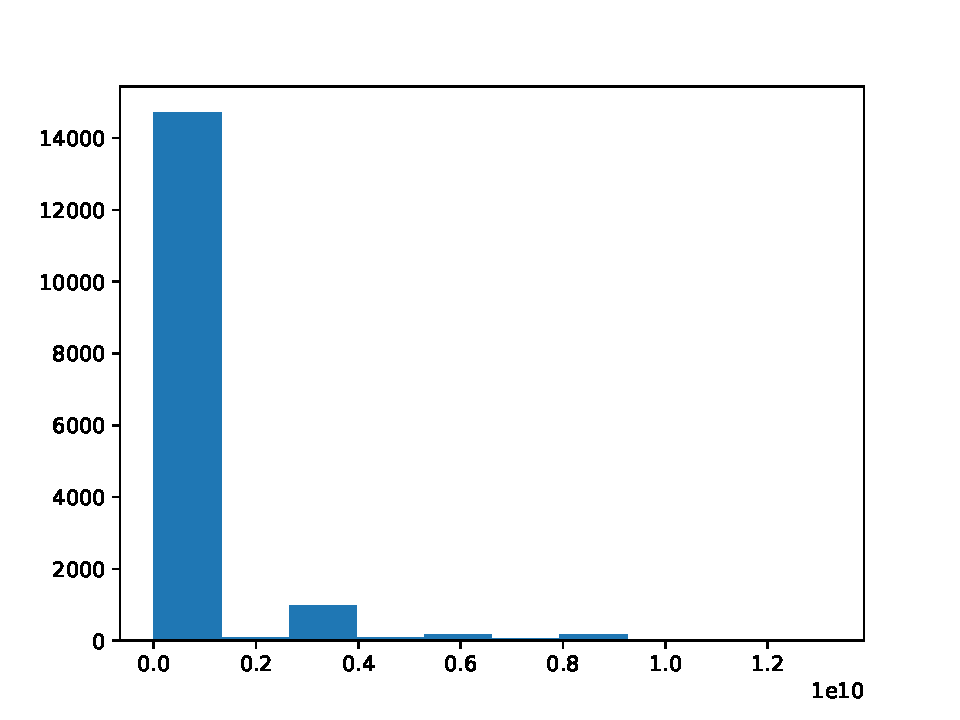
\includegraphics[width=\textwidth]{../../Output/Plots/brand_var.pdf}

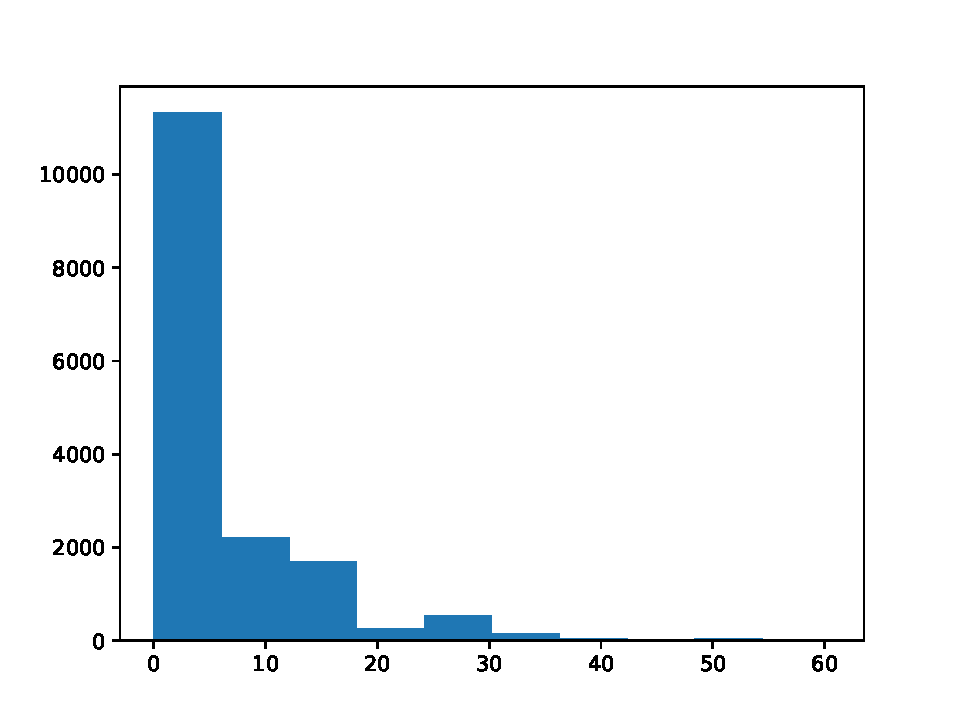
\includegraphics[width=\textwidth]{../../Output/Plots/flavor_var_hist.pdf}

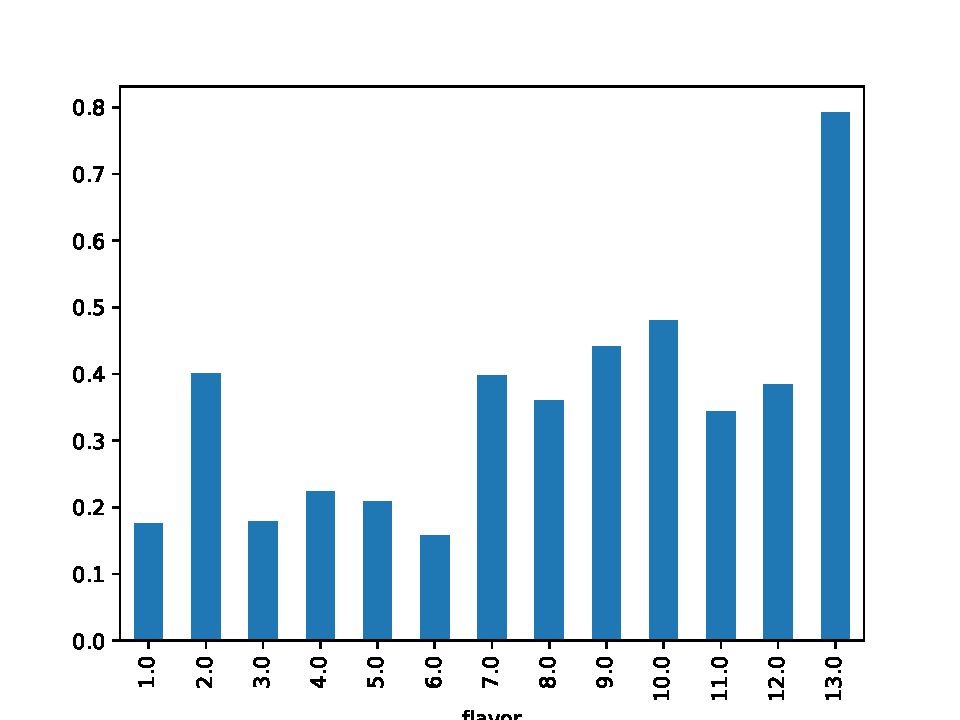
\includegraphics[width=\textwidth]{../../Output/Plots/repeat_flavor_bar.pdf}

The first plot shows the variance in brand choice within household across time. There is little variance here. The second shows variance in flavor choice within household and across time. Again, mostly centered at zero, thought there is more spread. However, looking at the third plot is where I think we see the most interesting pattern. Here, aside from plain yogurt (12), we see that the mean repeat purchase frequency is about 50\% or less for each flavor. This is remarkably similar to our Monte Carlo estimates, and shows the dynamics play a meaningful role, accounting for last period's impact on this one. 

\section{Next Steps}

I am still doing data testing, trying to get the right measure of variety. Further, I am working on other characteristics like protein content and whether it is a special yogurt like greek or skyr. This is textual in description variables, so have to parse quite a bit. Open to any feedback, especially on the plots. 

\end{document}
